\par Le membre du groupe responsable de cette partie était Emmanuel Guet.
\par Les armes définissent le gameplay du jeu, et n'importe quelle modification changerait radicalement la façon de jouer. C'est pourquoi les armes sont réellement très importants quant à la façon d'appréhender un niveau. Et oui, si vous échouez à un niveau, peut-être devriez vous repenser votre gestion de l'énergie et de vos armes. Voici la liste des armes dont le joueur dispose :


\begin{itemize}

\item[$\bullet$ Arme de base]
	\par~	
	\vspace{0.5cm}
	\par~
	\begin{itemize}
		\item Coût : 0
		\item Avantages : Aucun coût en énergie, est correct dans toutes les situations, peut être amélioré deux fois pour en faire une arme beaucoup plus forte, avec toujours aucun coût en énergie.
		\item Inconvénients : Arme très moyenne, il s'agit de l'arme de base du joueur, non faite pour faire tout un niveau avec. Si elle n'est pas améliorée, elle est encore plus faible.
		\item Bons contre : Polyvalent, mais moyen.
	\end{itemize}
	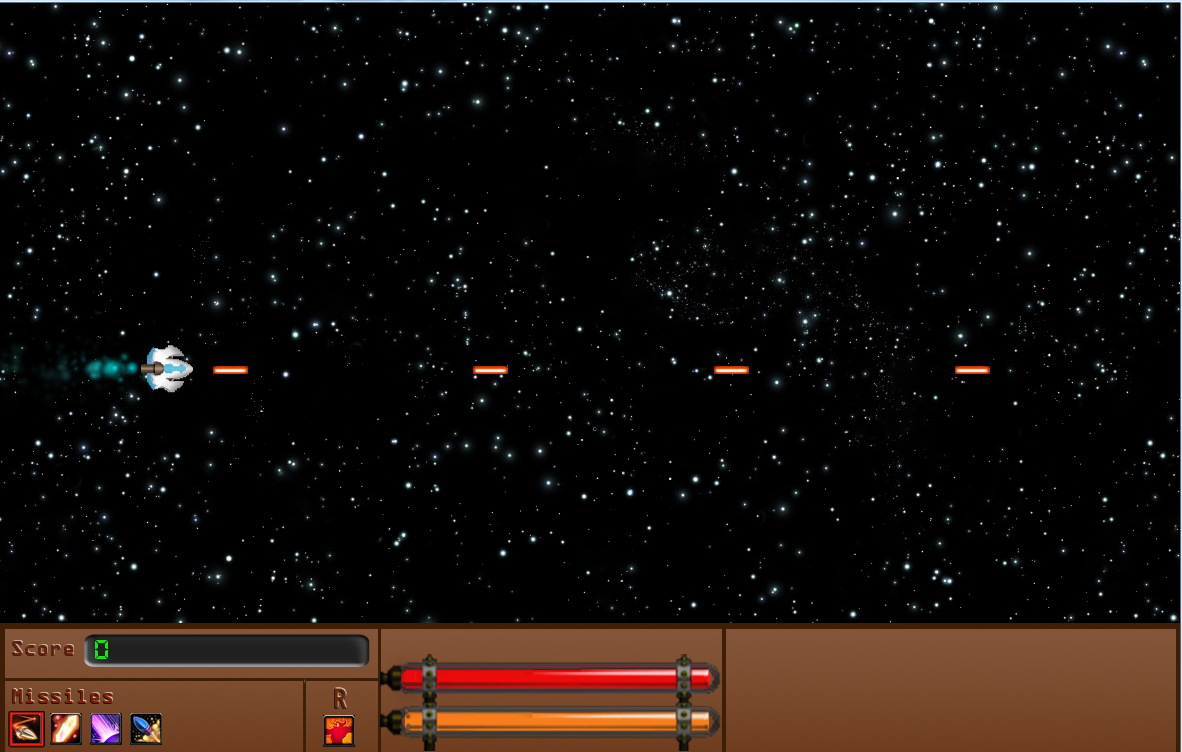
\includegraphics[width=11cm]{images/armes/base_1.png}
	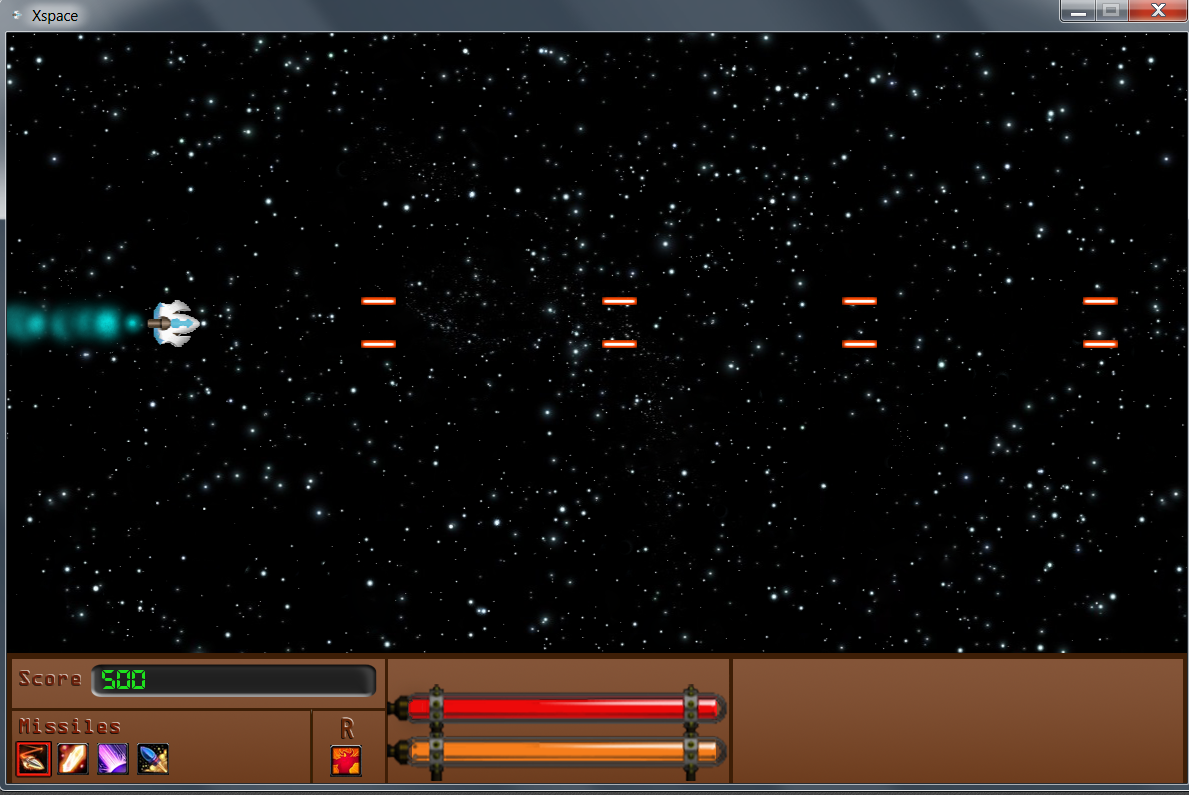
\includegraphics[width=11cm]{images/armes/base_2.png}
	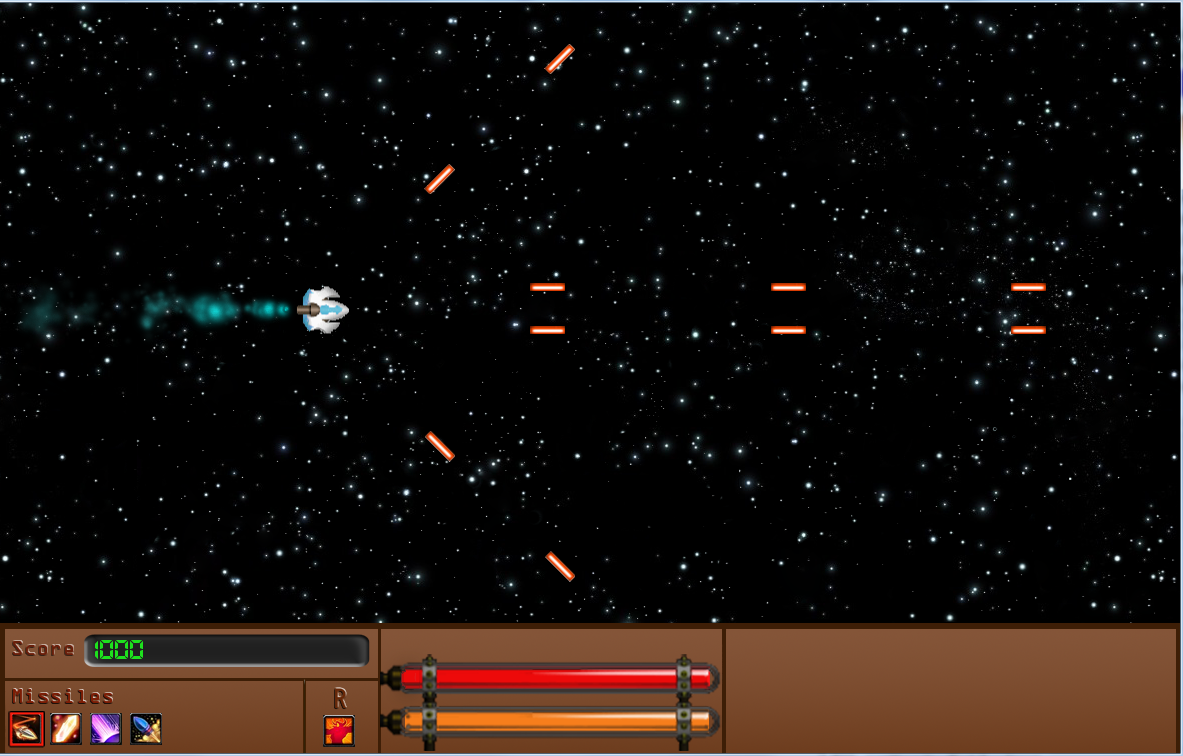
\includegraphics[width=11cm]{images/armes/base_3.png}

\item[$\bullet$ Tir Lourd]
	\par~	
	\vspace{0.5cm}
	\par~
	\begin{itemize}
		\item Coût : 100 points d'énergie par tir
		\item Avantages : Des dégâts à l'impact très élevé, capable de détruire instantanément la grande majorité des ennemis
		\item Inconvénients : Une vitesse vraiment lente, la taille n'est laser n'est pas énorme et cadence de tir faible, il est donc difficile de bien viser
		\item Bons contre : Ennemis très résistants – Boss
	\end{itemize}
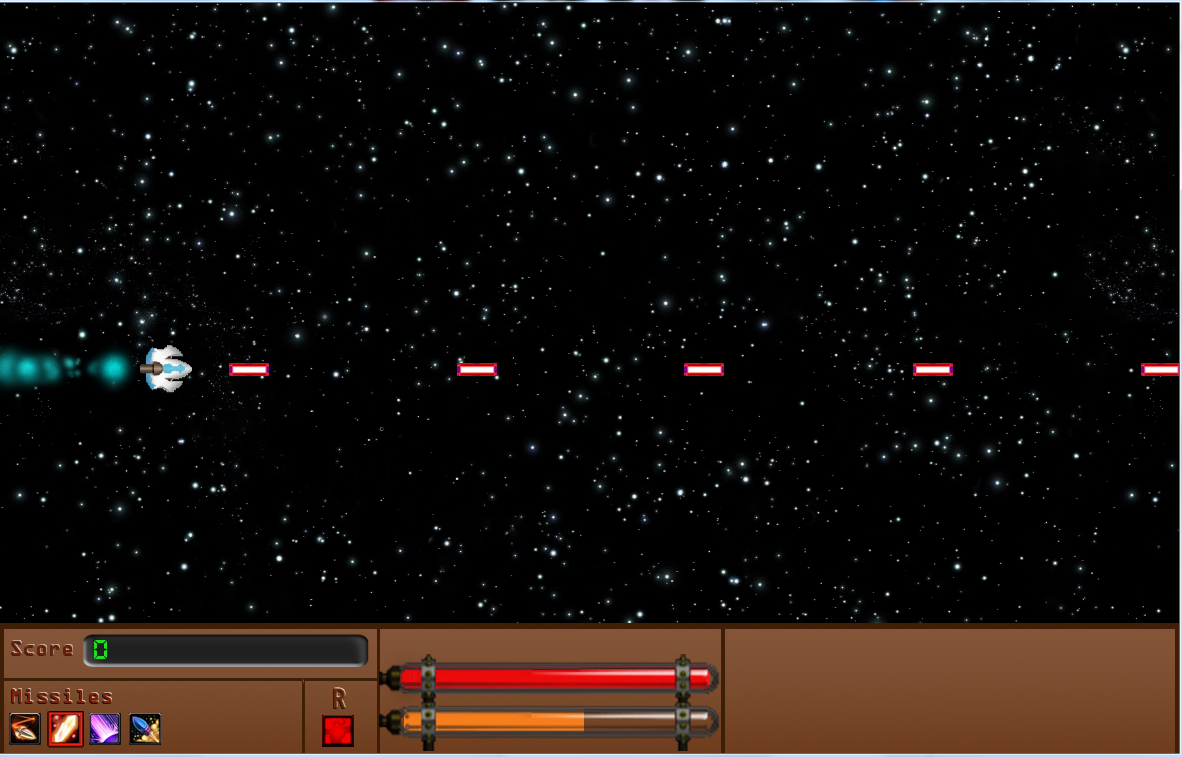
\includegraphics[width=11cm]{images/armes/heavy.png}
\item[$\bullet$ Laser]
	\par~
	\vspace{0.5cm}
	\par~
	\begin{itemize}
		\item Coût : 100 / 0,1s
		\item Avantages : Arme dévastatrice, détruit très rapidement les vaisseaux, permet d'infliger de gros dégâts à un boss, facile à utiliser. A la particularité de détruire aussi les missiles se trouvant sur son chemin
		\item Inconvénients : Un coût extrêmement élevé (vide une barre d'énergie pleine en une seconde)
		\item Bons contre : Tout.
	\end{itemize}
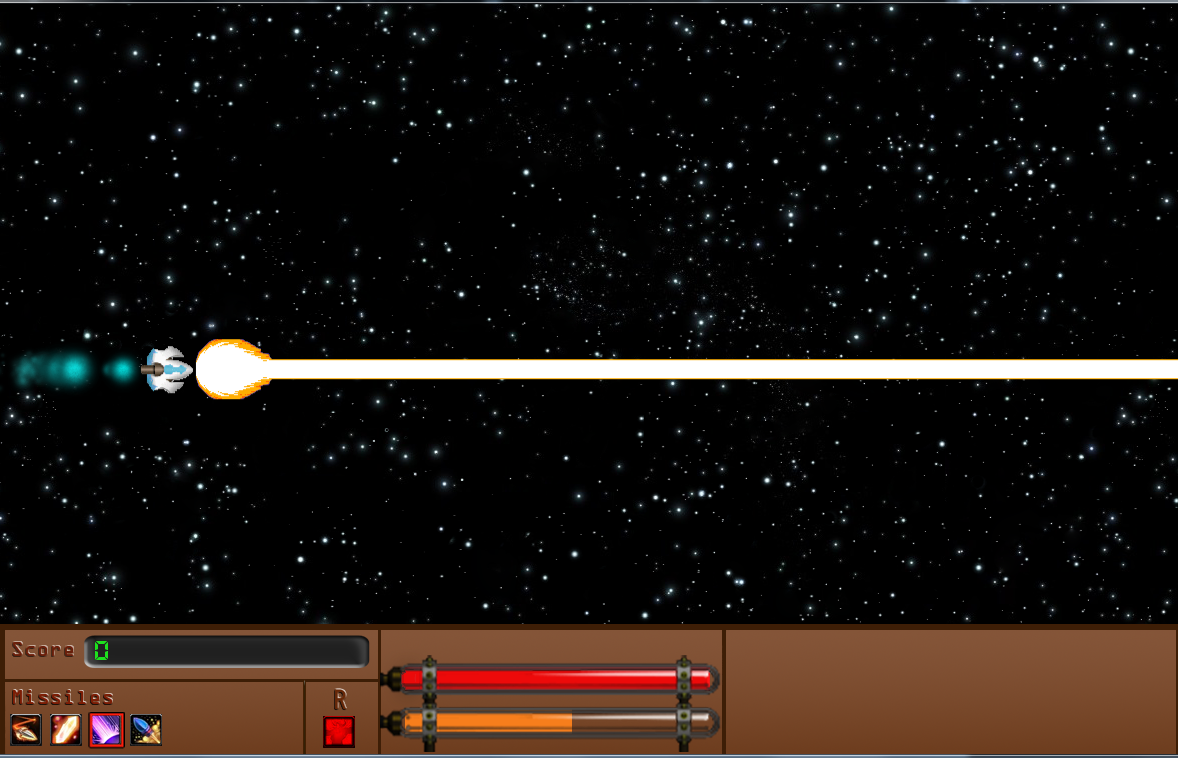
\includegraphics[width=11cm]{images/armes/laser.png}

\item[$\bullet$ Roquette]
	\par~
	\vspace{0.5cm}
	\par~
	\begin{itemize}
	\item Coût : 200
	\item Avantages : Vitesse du projectile élevée, bons dégâts à l'impact et arme à effet de zone : endommage tous les vaisseaux proches de l'explosion, le cas échéant les détruisant
	\item Inconvénients : Faible contre les ennemis isolés, demande beaucoup d'énergie à chaque tir
	\item Bons contre : Groupe d'ennemis
	\end{itemize}
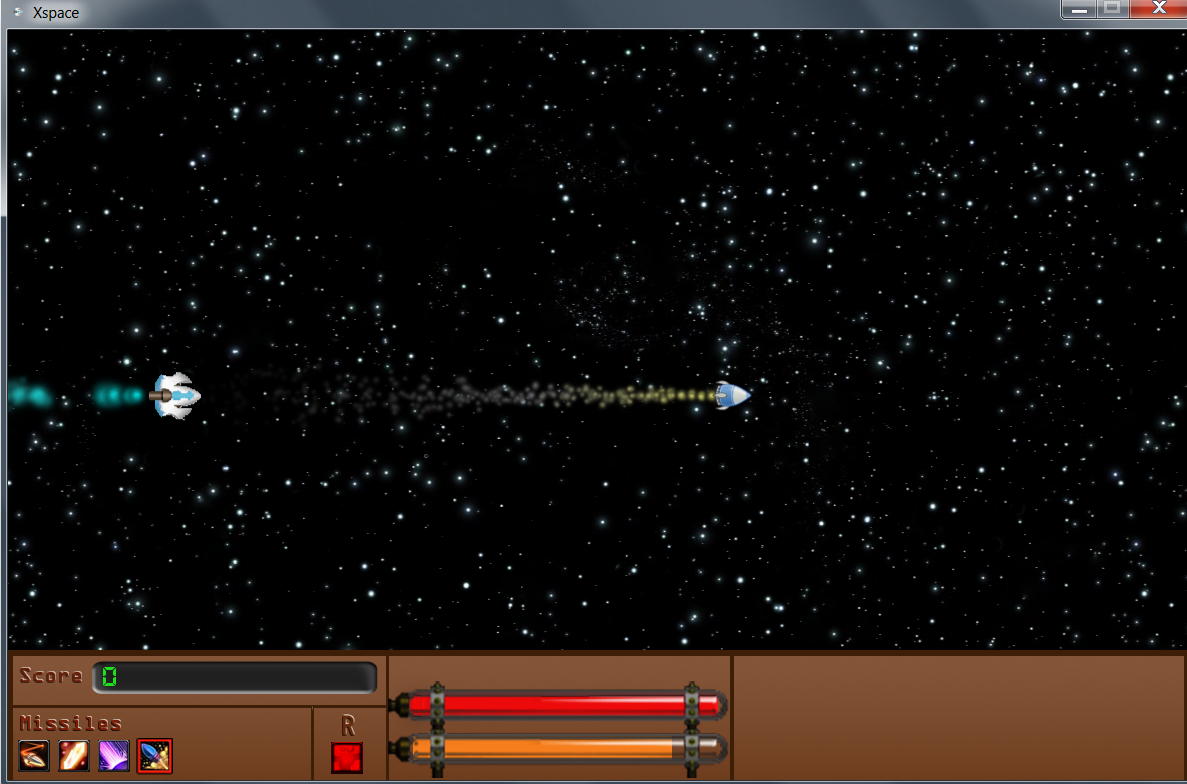
\includegraphics[width=11cm]{images/armes/roquette.png}
\end{itemize}

\par\par Cette seconde sous partie est consacrée aux différents bonus du jeu qui, rappelont le, peuvent-être récupérés sur des ennemis morts.

\begin{center}
\par 
\includegraphics{images/bonus/bonusVie.png} 
\par Rend 200 points de vie
\vspace{0.8cm}
\par 
\includegraphics{images/bonus/bonusScore.png} 
\par Donne 2000 points de score supplémentaires
\vspace{0.8cm}
\par \includegraphics{images/bonus/bonusEnergie.png}
\par Rend 500 points d'énergie (une demi barre)
\vspace{0.8cm}
\par 
\includegraphics{images/bonus/bonusBaseWeapon.png}
\par Améliore l'arme de base du joueur
\par 
\includegraphics{images/bonus/bonusSpeed.png} 
\par Augmente la vitesse de déplacement du joueur pendant 10 secondes
\vspace{0.8cm}
\par 
\includegraphics{images/bonus/bonusSpeedAttack.png} 
\par Augmente la vitesse de tir sur l'arme de base du joueur pendant 10 secondes
\vspace{0.8cm}
\end{center}